% Created by tikzDevice version 0.12.3.1 on 2022-03-10 11:32:07
% !TEX encoding = UTF-8 Unicode
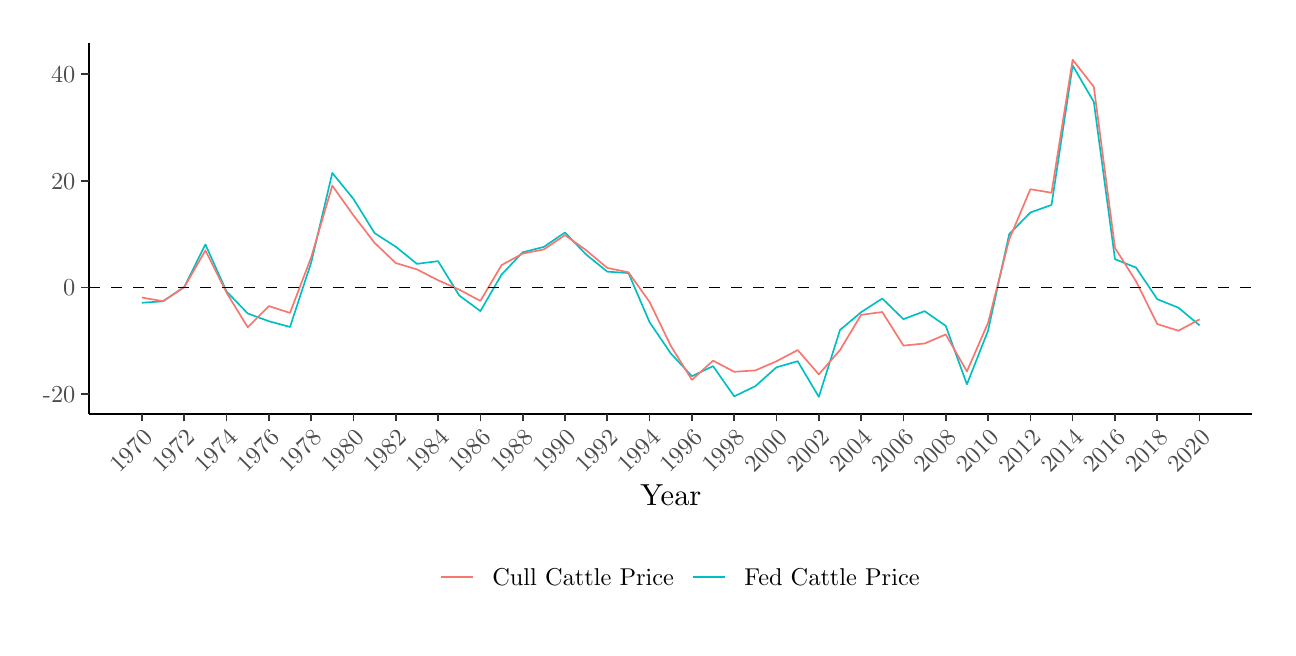
\begin{tikzpicture}[x=1pt,y=1pt]
\definecolor{fillColor}{RGB}{255,255,255}
\path[use as bounding box,fill=fillColor,fill opacity=0.00] (0,0) rectangle (448.07,216.81);
\begin{scope}
\path[clip] (  0.00,  0.00) rectangle (448.07,216.81);
\definecolor{drawColor}{RGB}{255,255,255}
\definecolor{fillColor}{RGB}{255,255,255}

\path[draw=drawColor,line width= 0.6pt,line join=round,line cap=round,fill=fillColor] (  0.00,  0.00) rectangle (448.07,216.81);
\end{scope}
\begin{scope}
\path[clip] ( 22.18, 77.31) rectangle (442.57,211.31);
\definecolor{fillColor}{RGB}{255,255,255}

\path[fill=fillColor] ( 22.18, 77.31) rectangle (442.57,211.31);
\definecolor{drawColor}{RGB}{0,191,196}

\path[draw=drawColor,line width= 0.6pt,line join=round] ( 41.29,117.40) --
	( 48.93,117.93) --
	( 56.58,123.14) --
	( 64.22,138.45) --
	( 71.86,121.49) --
	( 79.51,113.54) --
	( 87.15,110.74) --
	( 94.79,108.66) --
	(102.44,131.92) --
	(110.08,164.32) --
	(117.72,154.93) --
	(125.37,142.57) --
	(133.01,137.66) --
	(140.66,131.47) --
	(148.30,132.44) --
	(155.94,120.04) --
	(163.59,114.40) --
	(171.23,127.58) --
	(178.87,135.64) --
	(186.52,137.59) --
	(194.16,142.80) --
	(201.80,134.83) --
	(209.45,128.65) --
	(217.09,128.14) --
	(224.73,110.37) --
	(232.38, 99.11) --
	(240.02, 90.87) --
	(247.66, 94.52) --
	(255.31, 83.58) --
	(262.95, 87.27) --
	(270.59, 94.09) --
	(278.24, 96.28) --
	(285.88, 83.40) --
	(293.53,107.56) --
	(301.17,114.00) --
	(308.81,118.93) --
	(316.46,111.47) --
	(324.10,114.36) --
	(331.74,109.07) --
	(339.39, 87.93) --
	(347.03,107.31) --
	(354.67,142.18) --
	(362.32,150.03) --
	(369.96,152.75) --
	(377.60,203.14) --
	(385.25,189.97) --
	(392.89,133.16) --
	(400.53,130.10) --
	(408.18,118.69) --
	(415.82,115.63) --
	(423.47,109.24);
\definecolor{drawColor}{RGB}{248,118,109}

\path[draw=drawColor,line width= 0.6pt,line join=round] ( 41.29,119.27) --
	( 48.93,117.98) --
	( 56.58,123.04) --
	( 64.22,136.31) --
	( 71.86,121.05) --
	( 79.51,108.57) --
	( 87.15,116.21) --
	( 94.79,113.75) --
	(102.44,133.83) --
	(110.08,159.72) --
	(117.72,148.97) --
	(125.37,139.05) --
	(133.01,131.76) --
	(140.66,129.47) --
	(148.30,125.54) --
	(155.94,122.15) --
	(163.59,118.08) --
	(171.23,131.00) --
	(178.87,135.18) --
	(186.52,136.68) --
	(194.16,141.84) --
	(201.80,136.39) --
	(209.45,129.99) --
	(217.09,128.41) --
	(224.73,117.68) --
	(232.38,101.85) --
	(240.02, 89.55) --
	(247.66, 96.49) --
	(255.31, 92.46) --
	(262.95, 92.96) --
	(270.59, 96.27) --
	(278.24,100.31) --
	(285.88, 91.53) --
	(293.53,100.31) --
	(301.17,113.04) --
	(308.81,114.06) --
	(316.46,101.92) --
	(324.10,102.69) --
	(331.74,105.96) --
	(339.39, 92.61) --
	(347.03,110.14) --
	(354.67,140.32) --
	(362.32,158.44) --
	(369.96,157.16) --
	(377.60,205.22) --
	(385.25,195.41) --
	(392.89,137.24) --
	(400.53,125.09) --
	(408.18,109.71) --
	(415.82,107.30) --
	(423.47,111.41);
\definecolor{drawColor}{RGB}{0,0,0}

\path[draw=drawColor,line width= 0.6pt,dash pattern=on 4pt off 4pt ,line join=round] ( 22.18,122.97) -- (442.57,122.97);
\end{scope}
\begin{scope}
\path[clip] (  0.00,  0.00) rectangle (448.07,216.81);
\definecolor{drawColor}{RGB}{0,0,0}

\path[draw=drawColor,line width= 0.6pt,line join=round] ( 22.18, 77.31) --
	( 22.18,211.31);
\end{scope}
\begin{scope}
\path[clip] (  0.00,  0.00) rectangle (448.07,216.81);
\definecolor{drawColor}{gray}{0.30}

\node[text=drawColor,anchor=base east,inner sep=0pt, outer sep=0pt, scale=  0.88] at ( 17.23, 81.42) {-20};

\node[text=drawColor,anchor=base east,inner sep=0pt, outer sep=0pt, scale=  0.88] at ( 17.23,119.94) {0};

\node[text=drawColor,anchor=base east,inner sep=0pt, outer sep=0pt, scale=  0.88] at ( 17.23,158.46) {20};

\node[text=drawColor,anchor=base east,inner sep=0pt, outer sep=0pt, scale=  0.88] at ( 17.23,196.98) {40};
\end{scope}
\begin{scope}
\path[clip] (  0.00,  0.00) rectangle (448.07,216.81);
\definecolor{drawColor}{gray}{0.20}

\path[draw=drawColor,line width= 0.6pt,line join=round] ( 19.43, 84.45) --
	( 22.18, 84.45);

\path[draw=drawColor,line width= 0.6pt,line join=round] ( 19.43,122.97) --
	( 22.18,122.97);

\path[draw=drawColor,line width= 0.6pt,line join=round] ( 19.43,161.49) --
	( 22.18,161.49);

\path[draw=drawColor,line width= 0.6pt,line join=round] ( 19.43,200.01) --
	( 22.18,200.01);
\end{scope}
\begin{scope}
\path[clip] (  0.00,  0.00) rectangle (448.07,216.81);
\definecolor{drawColor}{RGB}{0,0,0}

\path[draw=drawColor,line width= 0.6pt,line join=round] ( 22.18, 77.31) --
	(442.57, 77.31);
\end{scope}
\begin{scope}
\path[clip] (  0.00,  0.00) rectangle (448.07,216.81);
\definecolor{drawColor}{gray}{0.20}

\path[draw=drawColor,line width= 0.6pt,line join=round] ( 41.29, 74.56) --
	( 41.29, 77.31);

\path[draw=drawColor,line width= 0.6pt,line join=round] ( 56.58, 74.56) --
	( 56.58, 77.31);

\path[draw=drawColor,line width= 0.6pt,line join=round] ( 71.86, 74.56) --
	( 71.86, 77.31);

\path[draw=drawColor,line width= 0.6pt,line join=round] ( 87.15, 74.56) --
	( 87.15, 77.31);

\path[draw=drawColor,line width= 0.6pt,line join=round] (102.44, 74.56) --
	(102.44, 77.31);

\path[draw=drawColor,line width= 0.6pt,line join=round] (117.72, 74.56) --
	(117.72, 77.31);

\path[draw=drawColor,line width= 0.6pt,line join=round] (133.01, 74.56) --
	(133.01, 77.31);

\path[draw=drawColor,line width= 0.6pt,line join=round] (148.30, 74.56) --
	(148.30, 77.31);

\path[draw=drawColor,line width= 0.6pt,line join=round] (163.59, 74.56) --
	(163.59, 77.31);

\path[draw=drawColor,line width= 0.6pt,line join=round] (178.87, 74.56) --
	(178.87, 77.31);

\path[draw=drawColor,line width= 0.6pt,line join=round] (194.16, 74.56) --
	(194.16, 77.31);

\path[draw=drawColor,line width= 0.6pt,line join=round] (209.45, 74.56) --
	(209.45, 77.31);

\path[draw=drawColor,line width= 0.6pt,line join=round] (224.73, 74.56) --
	(224.73, 77.31);

\path[draw=drawColor,line width= 0.6pt,line join=round] (240.02, 74.56) --
	(240.02, 77.31);

\path[draw=drawColor,line width= 0.6pt,line join=round] (255.31, 74.56) --
	(255.31, 77.31);

\path[draw=drawColor,line width= 0.6pt,line join=round] (270.59, 74.56) --
	(270.59, 77.31);

\path[draw=drawColor,line width= 0.6pt,line join=round] (285.88, 74.56) --
	(285.88, 77.31);

\path[draw=drawColor,line width= 0.6pt,line join=round] (301.17, 74.56) --
	(301.17, 77.31);

\path[draw=drawColor,line width= 0.6pt,line join=round] (316.46, 74.56) --
	(316.46, 77.31);

\path[draw=drawColor,line width= 0.6pt,line join=round] (331.74, 74.56) --
	(331.74, 77.31);

\path[draw=drawColor,line width= 0.6pt,line join=round] (347.03, 74.56) --
	(347.03, 77.31);

\path[draw=drawColor,line width= 0.6pt,line join=round] (362.32, 74.56) --
	(362.32, 77.31);

\path[draw=drawColor,line width= 0.6pt,line join=round] (377.60, 74.56) --
	(377.60, 77.31);

\path[draw=drawColor,line width= 0.6pt,line join=round] (392.89, 74.56) --
	(392.89, 77.31);

\path[draw=drawColor,line width= 0.6pt,line join=round] (408.18, 74.56) --
	(408.18, 77.31);

\path[draw=drawColor,line width= 0.6pt,line join=round] (423.47, 74.56) --
	(423.47, 77.31);
\end{scope}
\begin{scope}
\path[clip] (  0.00,  0.00) rectangle (448.07,216.81);
\definecolor{drawColor}{gray}{0.30}

\node[text=drawColor,rotate= 45.00,anchor=base east,inner sep=0pt, outer sep=0pt, scale=  0.88] at ( 45.57, 68.07) {1970};

\node[text=drawColor,rotate= 45.00,anchor=base east,inner sep=0pt, outer sep=0pt, scale=  0.88] at ( 60.86, 68.07) {1972};

\node[text=drawColor,rotate= 45.00,anchor=base east,inner sep=0pt, outer sep=0pt, scale=  0.88] at ( 76.15, 68.07) {1974};

\node[text=drawColor,rotate= 45.00,anchor=base east,inner sep=0pt, outer sep=0pt, scale=  0.88] at ( 91.44, 68.07) {1976};

\node[text=drawColor,rotate= 45.00,anchor=base east,inner sep=0pt, outer sep=0pt, scale=  0.88] at (106.72, 68.07) {1978};

\node[text=drawColor,rotate= 45.00,anchor=base east,inner sep=0pt, outer sep=0pt, scale=  0.88] at (122.01, 68.07) {1980};

\node[text=drawColor,rotate= 45.00,anchor=base east,inner sep=0pt, outer sep=0pt, scale=  0.88] at (137.30, 68.07) {1982};

\node[text=drawColor,rotate= 45.00,anchor=base east,inner sep=0pt, outer sep=0pt, scale=  0.88] at (152.58, 68.07) {1984};

\node[text=drawColor,rotate= 45.00,anchor=base east,inner sep=0pt, outer sep=0pt, scale=  0.88] at (167.87, 68.07) {1986};

\node[text=drawColor,rotate= 45.00,anchor=base east,inner sep=0pt, outer sep=0pt, scale=  0.88] at (183.16, 68.07) {1988};

\node[text=drawColor,rotate= 45.00,anchor=base east,inner sep=0pt, outer sep=0pt, scale=  0.88] at (198.45, 68.07) {1990};

\node[text=drawColor,rotate= 45.00,anchor=base east,inner sep=0pt, outer sep=0pt, scale=  0.88] at (213.73, 68.07) {1992};

\node[text=drawColor,rotate= 45.00,anchor=base east,inner sep=0pt, outer sep=0pt, scale=  0.88] at (229.02, 68.07) {1994};

\node[text=drawColor,rotate= 45.00,anchor=base east,inner sep=0pt, outer sep=0pt, scale=  0.88] at (244.31, 68.07) {1996};

\node[text=drawColor,rotate= 45.00,anchor=base east,inner sep=0pt, outer sep=0pt, scale=  0.88] at (259.59, 68.07) {1998};

\node[text=drawColor,rotate= 45.00,anchor=base east,inner sep=0pt, outer sep=0pt, scale=  0.88] at (274.88, 68.07) {2000};

\node[text=drawColor,rotate= 45.00,anchor=base east,inner sep=0pt, outer sep=0pt, scale=  0.88] at (290.17, 68.07) {2002};

\node[text=drawColor,rotate= 45.00,anchor=base east,inner sep=0pt, outer sep=0pt, scale=  0.88] at (305.45, 68.07) {2004};

\node[text=drawColor,rotate= 45.00,anchor=base east,inner sep=0pt, outer sep=0pt, scale=  0.88] at (320.74, 68.07) {2006};

\node[text=drawColor,rotate= 45.00,anchor=base east,inner sep=0pt, outer sep=0pt, scale=  0.88] at (336.03, 68.07) {2008};

\node[text=drawColor,rotate= 45.00,anchor=base east,inner sep=0pt, outer sep=0pt, scale=  0.88] at (351.32, 68.07) {2010};

\node[text=drawColor,rotate= 45.00,anchor=base east,inner sep=0pt, outer sep=0pt, scale=  0.88] at (366.60, 68.07) {2012};

\node[text=drawColor,rotate= 45.00,anchor=base east,inner sep=0pt, outer sep=0pt, scale=  0.88] at (381.89, 68.07) {2014};

\node[text=drawColor,rotate= 45.00,anchor=base east,inner sep=0pt, outer sep=0pt, scale=  0.88] at (397.18, 68.07) {2016};

\node[text=drawColor,rotate= 45.00,anchor=base east,inner sep=0pt, outer sep=0pt, scale=  0.88] at (412.46, 68.07) {2018};

\node[text=drawColor,rotate= 45.00,anchor=base east,inner sep=0pt, outer sep=0pt, scale=  0.88] at (427.75, 68.07) {2020};
\end{scope}
\begin{scope}
\path[clip] (  0.00,  0.00) rectangle (448.07,216.81);
\definecolor{drawColor}{RGB}{0,0,0}

\node[text=drawColor,anchor=base,inner sep=0pt, outer sep=0pt, scale=  1.10] at (232.38, 44.09) {Year};
\end{scope}
\begin{scope}
\path[clip] (  0.00,  0.00) rectangle (448.07,216.81);
\definecolor{fillColor}{RGB}{255,255,255}

\path[fill=fillColor] (136.94,  5.50) rectangle (327.81, 30.95);
\end{scope}
\begin{scope}
\path[clip] (  0.00,  0.00) rectangle (448.07,216.81);
\definecolor{drawColor}{RGB}{248,118,109}

\path[draw=drawColor,line width= 0.6pt,line join=round] (149.39, 18.23) -- (160.95, 18.23);
\end{scope}
\begin{scope}
\path[clip] (  0.00,  0.00) rectangle (448.07,216.81);
\definecolor{drawColor}{RGB}{248,118,109}

\path[draw=drawColor,line width= 0.6pt,line join=round] (149.39, 18.23) -- (160.95, 18.23);
\end{scope}
\begin{scope}
\path[clip] (  0.00,  0.00) rectangle (448.07,216.81);
\definecolor{drawColor}{RGB}{0,191,196}

\path[draw=drawColor,line width= 0.6pt,line join=round] (240.48, 18.23) -- (252.05, 18.23);
\end{scope}
\begin{scope}
\path[clip] (  0.00,  0.00) rectangle (448.07,216.81);
\definecolor{drawColor}{RGB}{0,191,196}

\path[draw=drawColor,line width= 0.6pt,line join=round] (240.48, 18.23) -- (252.05, 18.23);
\end{scope}
\begin{scope}
\path[clip] (  0.00,  0.00) rectangle (448.07,216.81);
\definecolor{drawColor}{RGB}{0,0,0}

\node[text=drawColor,anchor=base west,inner sep=0pt, outer sep=0pt, scale=  0.88] at (167.90, 15.20) {Cull Cattle Price};
\end{scope}
\begin{scope}
\path[clip] (  0.00,  0.00) rectangle (448.07,216.81);
\definecolor{drawColor}{RGB}{0,0,0}

\node[text=drawColor,anchor=base west,inner sep=0pt, outer sep=0pt, scale=  0.88] at (258.99, 15.20) {Fed Cattle Price};
\end{scope}
\end{tikzpicture}
